% !TEX root = ../thesis_main.tex

\section{Validation of \pygbe and Replication of Ellis et al. 2016  et al 2005} \label{chap:rep_val_ellis}
\graphicspath{{replication_validation/figs/}}

The work of Ellis et al. "Aspect-ratio driven evolution of high-order resonant modes and near-field distributions in
localized surface phonon polariton nanostructures." \cite{ellis2016} has both computational and experimental results, what makes 
it a perfect candidate to perform a validation as well as a replication study. Ellis and coworkers study the excitation of 
multipolar localized surface polaritons (SPhP), by computing and measuring the polarized reflectance on 4H-SiC pillars of
fixed width ($W = 400$ nm), fixed hight ($H=950$ nm) and varied length ($L=400-4800$ nm). To reduce coupling these pillars are 
pattern on a square grid with $P = L + 500$ nm. In their experiments (simulations), they measure (compute) the polarized reflectance
where the incident polarization is oriented parallel or perpendicular to the length ($L$) of the pillars.
We started by replicating a computational result shown in Figure S4 of their supplementary material. Figure S4 of the 
supplementary material shows simulation results for the resonance spectral position of the lower frequency mode when the angle of 
incidence is 22 degrees and the polarization is parallel to the length of the pillars. They present results for separations of $500$ nm 
(red curve) and $5000$ (black curve), being the latter a good candidate for replication with \pygbe since a larger gap diminishes 
the coupling (not included in our model). The setup in our computations consists of a single pillar with no substrate.
Secondly, we aimed to replicate the results of Figure 2a of the main paper, 
corresponding to reflectance measurements across the wave number for pillars of aspect ratio $AR=4$, angle of incidence 22 degrees, 
and incoming parallel polarization. Since for this the authors also reported experimental results we decided to us them for the 
validation of our solver.
For all the simulations involved in the replication and validation studies we use experimental values of the complex dielectric data 
for 4H-SIC provided by the authors of Ellis et al. via private communication. 

\textbf{Differences in method and input data}

\begin{itemize}

\item {The simulations of Ellis et al. compute the solution of the Maxwell's equations using the RF package
of the finite element solver in the commercial software COMSOL. Their setup consists of one pillar over a 
substrate, with periodic boundary conditions to emulate the array of pillar used in their experiments. In our 
solver we use a boundary element method in the quasistatic approximation, which is suitable since the wavelengths
involved are in the range $10000-12500$ nm, and are considerably larger than the pillar's dimensions. We compute 
the extinction cross section, where the resonance express as peaks instead of dips as in the reflection plots of 
Ellis et al. The intensity of the peaks is not comparable, however, we are looking to match the wave number at which
they happen}

\item {The simulations of Ellis et al. rely on a volumetric model and therefore it uses a volumetric mesh. In our 
solver the geometries are represented as a triangular surface meshes. For the validation and replication of Figure 2a of 
their paper, where the pillars have an aspect ratio of $AR=4$, we use a non-uniform triangular mesh ($N=4398$) that 
was provided by the authors of Ellis et al. However, for the replication of the Figure S4 of the supplementary material, 
we were missing the remaining meshes for the other aspect ratios. To overcome this, we generated the meshes with our Python 
script, and we determined the density to be used by comparing simulations for the case of aspect ratio $AR=4$ of our mesh and 
the one provided by Ellis and coworkers. Using approximately double the number of elements ($N=8564$) than the original mesh 
and rounding the edges using Trimesh, the relative errors for the extinction cross-section were, on average, smaller than 
$3\%$, and the variations on the wave number of the peak position was smaller than $1$cm$^-1$. After this analysis we 
concluded in a density of $\approx \; 1.7 \times10^{-5}$ triangles per $\text{\AA}$ squared, which we used to create the meshes
for the remaining aspect ratio geometries.}

\item {In Ellis et al. they perform simulations for different angles of incidence of the illuminating vector. To achieve this 
using \pygbe we rotated the geometry, since the direction of the illuminating vector in our solver is fixed.}
\end{itemize}

\subsection{Replication of Figure S4 of supplementary material of Ellis et al. 2016}

To replicate Figure S4 of teh supplementary material we needed to identify the lower-frequency mode for every different 
aspect ratio in our computations. For the values of aspect ratio ($AR$) from 1 to 7, we computed the extinction cross section 
$C_{ext}$ across wave numbers in the range of $800-1000$ cm$^{-1}$, and we identified the lower-frequency mode 
($E^{\parallel}_{100}$ for Ellis et al.) that was not a longitudinal mode. The longitudinal modes are the ones associated with 
the height of the pillar and they appear only when we have an angle of incidence that is off-normal. 
Figure \ref{fig:AR_22_vs_norm} shows the results of the extinction cross-section of a SiC pillar for different values of 
length ($L=400$-$2800$ nm), for normal and 22-degrees angle of incidence (see Figure \ref{fig:ellis_ang_inc}). We performed 
the simulations for the long-edge orientation, meaning that the electric field is aligned with the length of the pillar when having a normal 
incidence. From each result of Figure \ref{fig:AR_22_vs_norm}, we selected the lowest non-longitudinal mode and extracted the corresponding wavelength
(see Table \ref{tab:ar_peaks}) to replicate Figure S4 of the supplementary material of Ellis et al. Figure \ref{fig:rep_FS4_ellis} shows the
results from Ellis et al. (obtained using the WebPlotDigitizer) and the results obtained using \pygbe. Table \ref{tab:err_AR} contains the 
percentage error and we can see that is below 2$\%$ for all the cases.

\begin{figure}
    \centering
    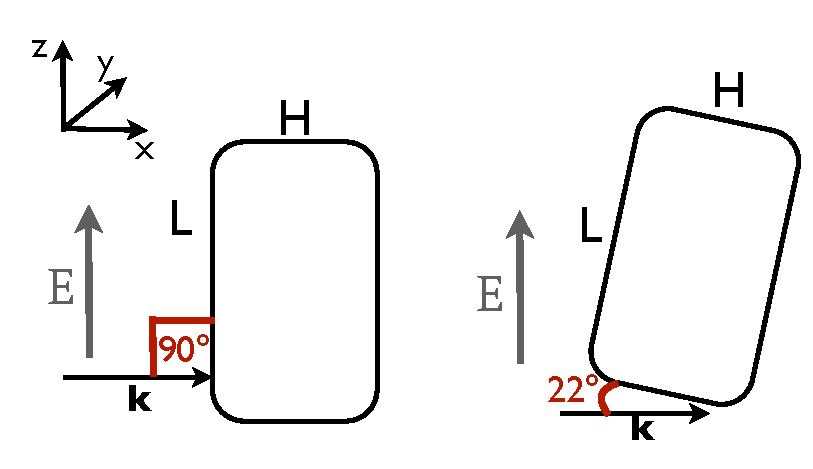
\includegraphics[width=0.45\textwidth]{ellis_ang_inc.pdf} 
    \caption{Diagram showing the angles of incidence in our simulation setups to comply with the configuration in the case from Ellis et al.}
    \label{fig:ellis_ang_inc}
\end{figure}

\begin{figure}
    \centering
    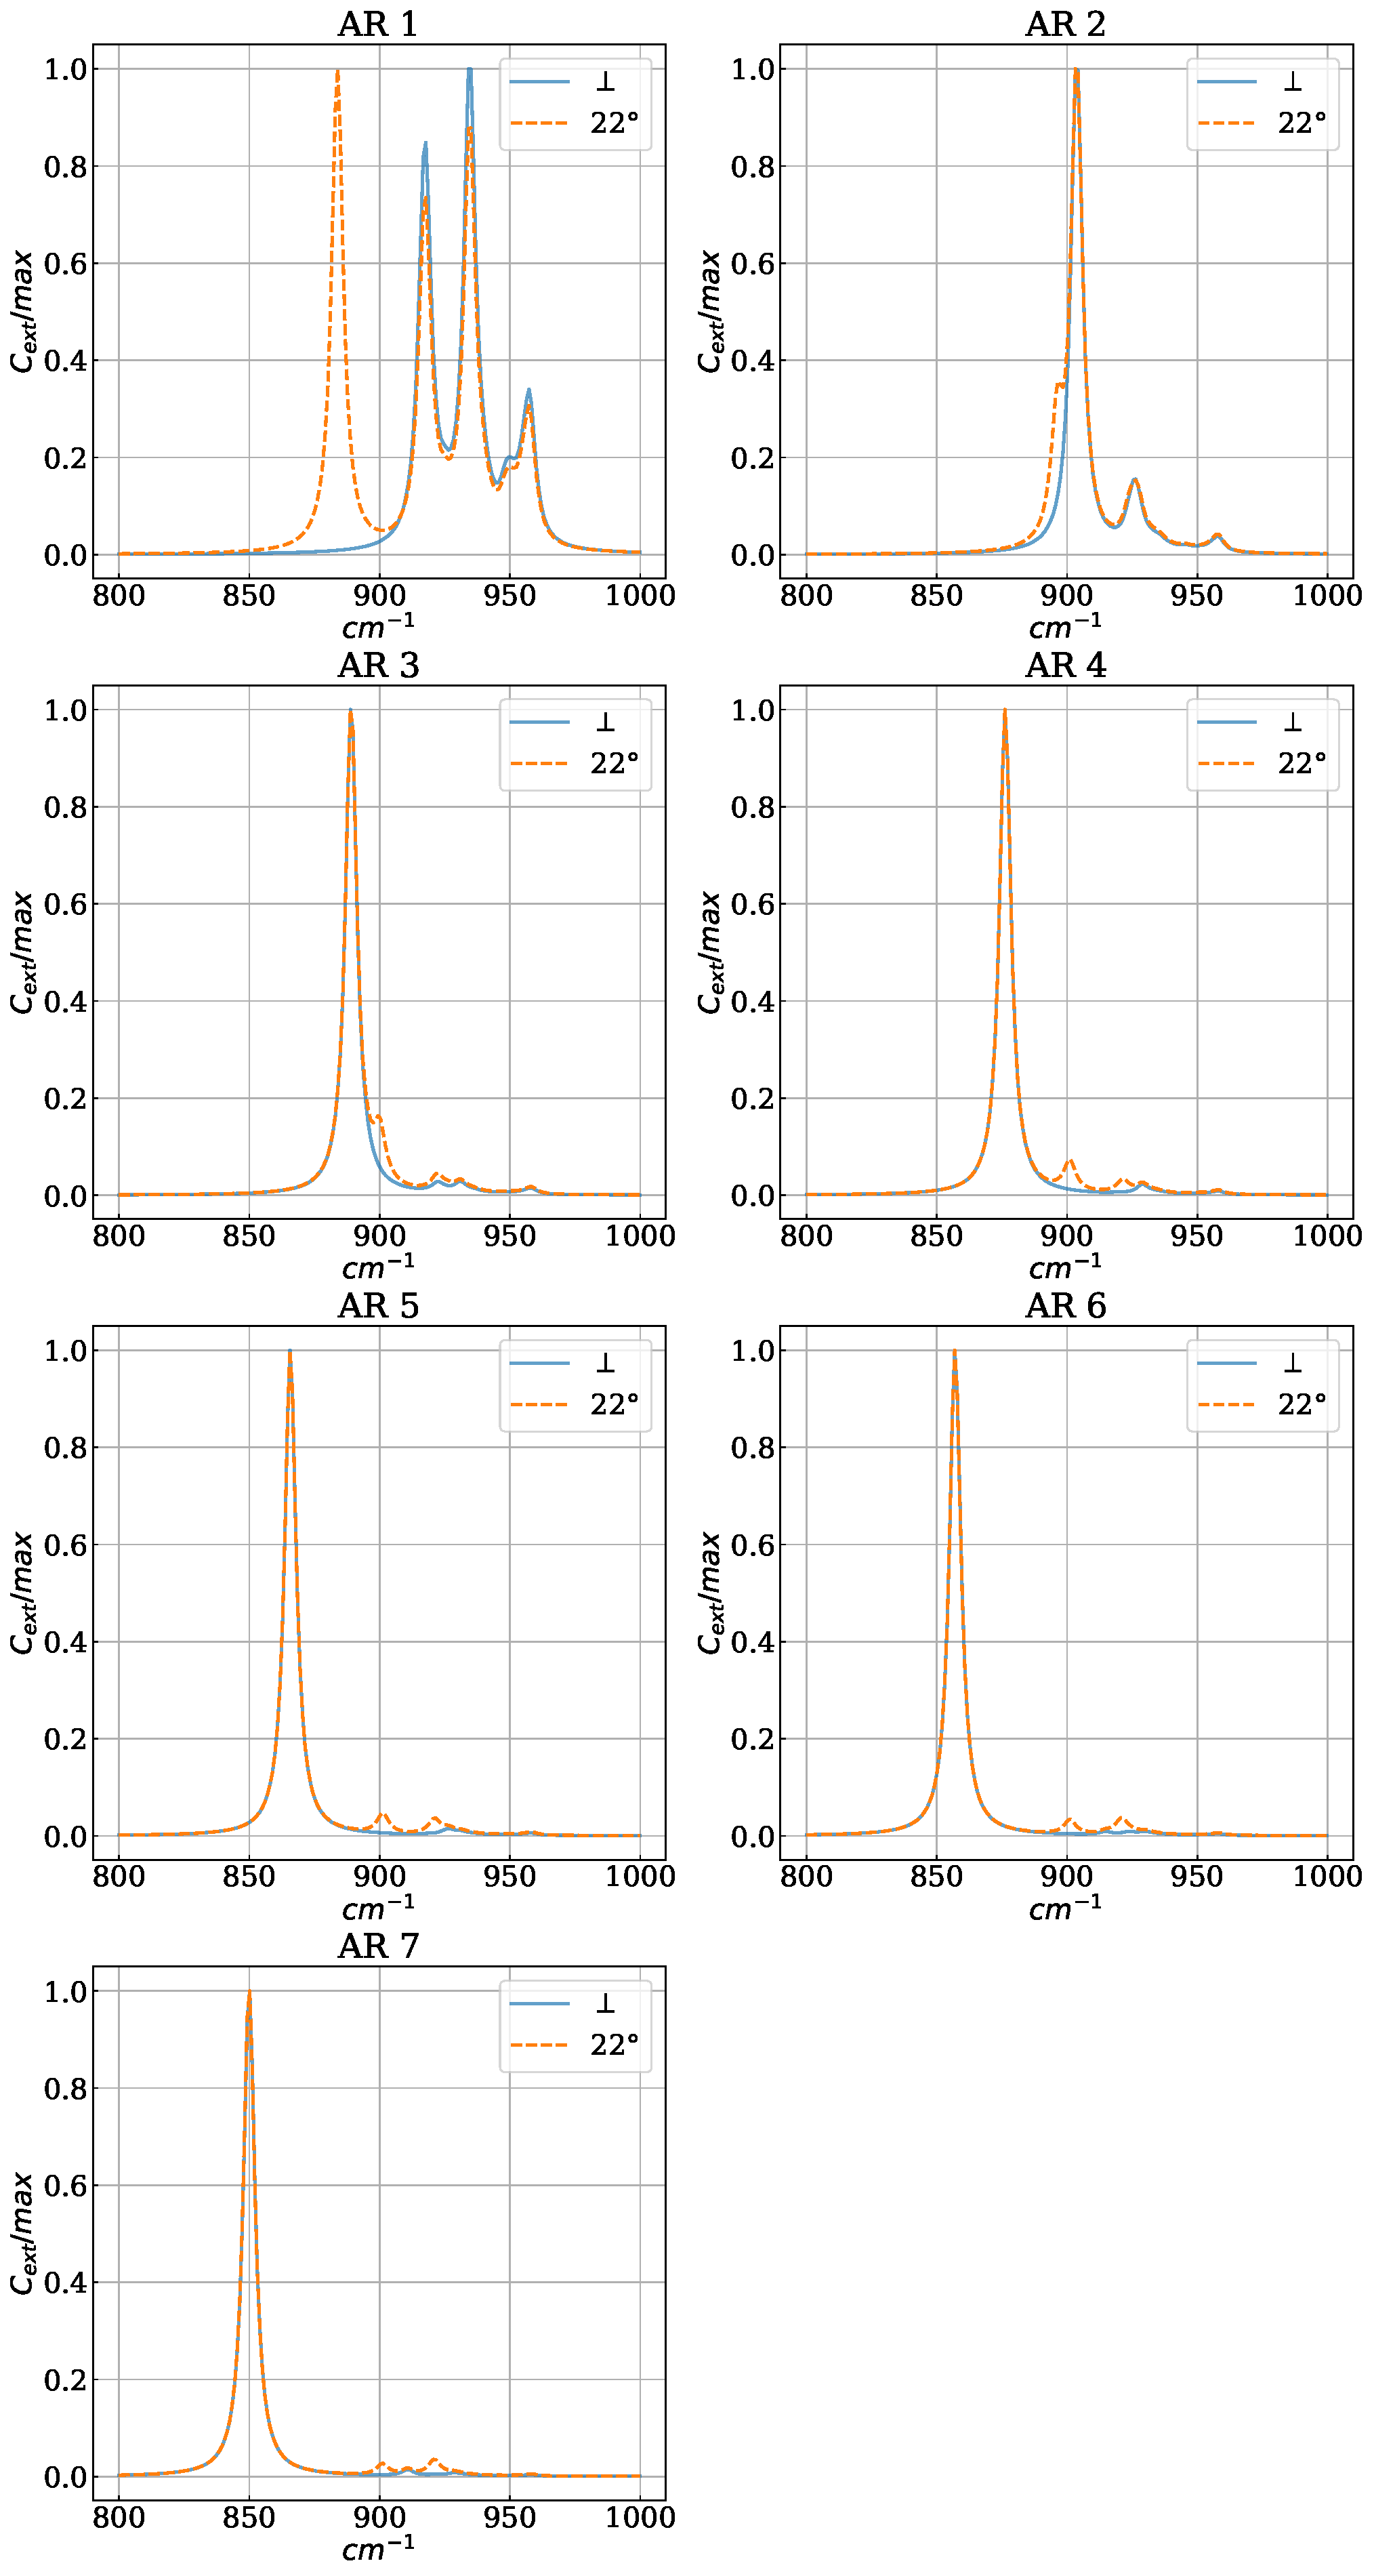
\includegraphics[width=0.72\textwidth]{AR_22_vs_norm.pdf} 
    \caption{Extinction cross-section across wave numbers for SiC pillars of varying aspect ratios,  
             ($H=950$ nm, $W=400$ nm, $L=400$--$2800$ nm, $AR=1$--$7$), with both normal incidence and a 
             22-degree incidence.}
    \label{fig:AR_22_vs_norm}
\end{figure}

\begin{table}
    \centering
      \caption{Wavelength at which peaks happen for different aspect ratios, for runs where the electric
      field is parallel to the length ($L$) of the pillar. We have normal incidence and 22-degree incidence.}
      \label{tab:ar_peaks}
      \begin{tabular}{c c c c c c c c}
        \textbf{AR} \\
        \hline
        \multirow{2}{*}{1} & $\perp$ & \textbf{917.73} & 934.092 & 949.604 & 957.325 \\ % <-- Combining 2 rows with arbitrary with (*) and content 12
        & 22$^{\circ}$ & 883.926 & \textbf{917.73} & 935.052 & 949.604 & 957.325 \\ % <-- Content of first column omitted.
        \hline
        \multirow{2}{*}{2} & $\perp$ & \textbf{903.233} & 926.395 & 944.762 & 958.242 \\ % <-- Combining 2 rows with arbitrary with (*) and content 12
        & 22$^{\circ}$ & 896.517 & \textbf{903.233} & 926.395 & 944.762 & 958.242 \\ % <-- Content of first column omitted.
        \hline
        \multirow{2}{*}{3} & $\perp$ & \textbf{888.793} & 922.552 & 931.223 & 948.613 & 958.242 \\ % <-- Combining 2 rows with arbitrary with (*) and content 12
        & 22$^{\circ}$ & \textbf{888.793} & 899.418 & 922.552 & 931.223 & 958.242 \\ % <-- Content of first column omitted.
        \hline
        \multirow{2}{*}{4} & $\perp$ & \textbf{876.186} & 929.32 & 946.639 & 958.242 \\ % <-- Combining 2 rows with arbitrary with (*) and content 12
        & 22$^{\circ}$ & \textbf{876.186} & 901.281 & 921.618 & 929.32 & 945.745 & 958.242 \\ % <-- Content of first column omitted.
        \hline
        \multirow{2}{*}{5} & $\perp$ & \textbf{865.576} & 926.395 & 945.745 & 958.242 \\ % <-- Combining 2 rows with arbitrary with (*) and content 12
        & 22$^{\circ}$ & \textbf{865.576} & 901.281 & 921.618 & 958.242 \\ % <-- Content of first column omitted.
        \hline
        \multirow{2}{*}{6} & $\perp$ &  \textbf{856.904} & 914.793 & 923.489 & 929.32 & 946.639 & 958.242\\ % <-- Combining 2 rows with arbitrary with (*) and content 12
        & 22$^{\circ}$ & \textbf{856.904} & 901.281 & 920.6 & 958.242\\ % <-- Content of first column omitted.
        \hline
        \multirow{2}{*}{7} & $\perp$ &  \textbf{850.134} & 910.963 & 921.618 & 928.372 & 946.639 & 958.242 \\ % <-- Combining 2 rows with arbitrary with (*) and content 12
        & 22$^{\circ}$ & \textbf{850.134} & 901.281 & 910.963 & 920.6 & 958.242\\ % <-- Content of first column omitted.
        \hline
      \end{tabular}
\end{table}

\begin{figure}
    \centering
    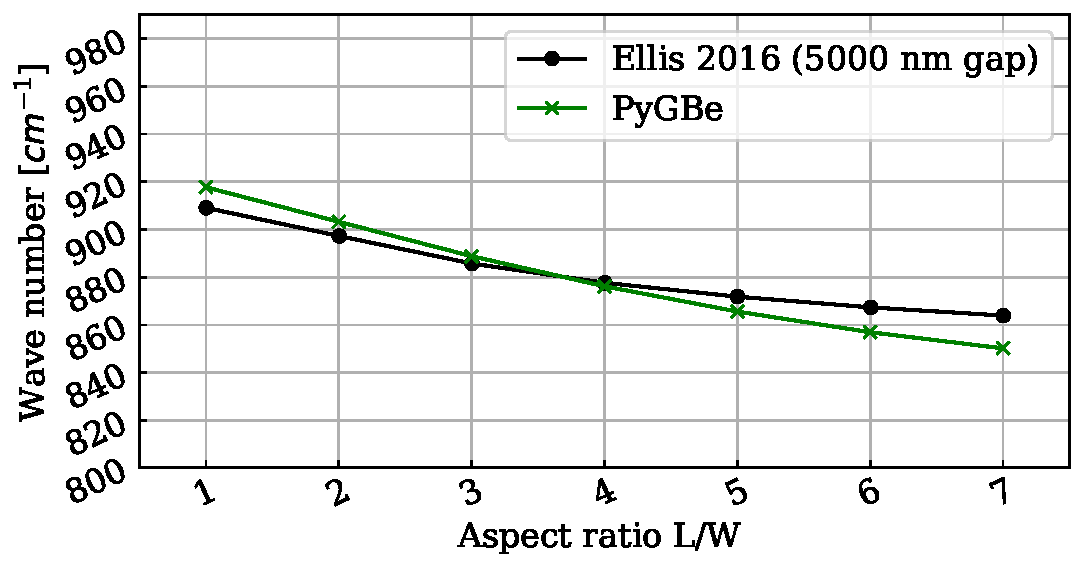
\includegraphics[width=0.85\textwidth]{AR_rep_FS4_Ellis2016.pdf} 
    \caption{Replication of figure S4 in the supplementary materials of Ellis et al., 2016. Wave
    number at which the $E^{\parallel}_{100}$ mode happens for different aspect ratios.}
    \label{fig:rep_FS4_ellis}
 \end{figure}
 
 \begin{table}
    \centering
    \caption{Percentage error for different aspect ratios.} 
    \label{tab:err_AR}
    \begin{tabular}{c c}
    \hline%\toprule
    AR & \% error \\
    \hline%\midrule
     $1$ & $0.95$ \\
     $2$ & $0.67$ \\
     $3$ & $0.35$ \\
     $4$ & $0.16$ \\
     $5$ & $0.72$ \\
     $6$ & $1.20$ \\
     $7$ & $1.59$ \\
    \hline%\bottomrule
    \end{tabular}
\end{table}


